 Let $\vec{O}$ be the centre of the circle and $r$ be the radius of the circle. Since centre lies on the given line
\begin{align}
\myvec{1&-3}\vec{O} = 11
\label{eq:4.2.7_eq1}
\end{align}
 Also 
\begin{align}
\norm{\vec{P} - \vec{O}}^2 = \norm{\vec{Q}- \vec{O}}^2 &= r^2 
\\
\implies 
\myvec{6&4}\vec{O} = 11
\label{eq:4.2.7_eq2}
\end{align}

From \eqref{eq:4.2.7_eq1} and \eqref{eq:4.2.7_eq2}, 
\begin{align}
\myvec{1&-3\\6&4}\vec{O} &= \myvec{11\\11} \\
\implies 
\vec{O} &= \myvec{\frac{7}{2}\\\frac{-5}{2}}
\end{align}
From  $\vec{O}$ we get $r$= 5.7.
This is verified in Fig. \ref{fig:4.2.7} by the following python code.
\begin{lstlisting}
solutions/7/codes/circle/circle.py
\end{lstlisting}
\begin{figure}[!ht]
\centering
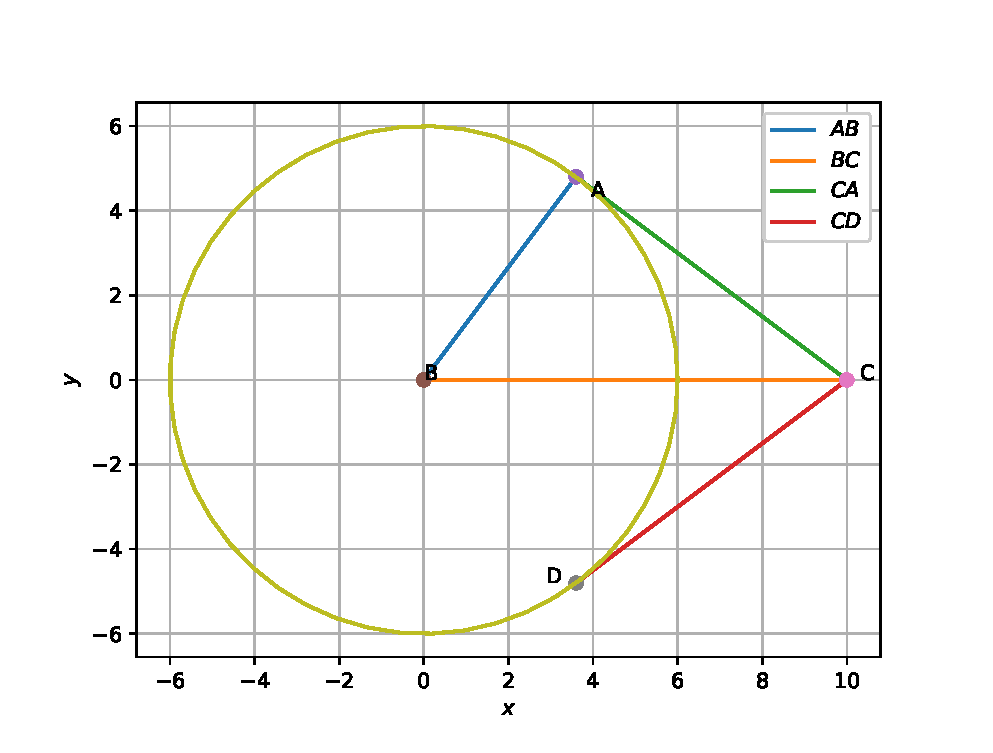
\includegraphics[width= \columnwidth]{./solutions/7/figs/circle/circle.eps}
\caption{}
\label{fig:4.2.7}
\end{figure}


